\documentclass[11pt]{article}
\usepackage[utf8]{inputenc}
\usepackage{graphicx}
\usepackage[left=2.5cm,top=2.5cm,right=2.5cm,bottom=2.5cm]{geometry}
\usepackage{times} % font type
\usepackage{url} % for clickable web addresses in PDF document
\usepackage{graphicx} % for figures
\usepackage{float} % to force figure or table here [H]
\usepackage{multirow} % For tables with different rows and columns
\usepackage{lipsum}  % for placeholder text (lorem ipsum ...)
%\usepackage{biblatex}

\title{Precision medicine and quantitative imaging in glioblastoma}
\author{ELMED219 (Artificial Intelligence and Computational Medicine), January 3-8, 2022\\
{\footnotesize \url{https://github.com/MMIV-ML/ELMED219-2022}}}

\date{Team \#k}
\begin{document}

\maketitle

\begin{scriptsize}
\begin{verbatim}
Team #k members:

Name, Category, E-mail	
NN, MED, nn@student.uib.no
MM, TEK, mm@student.uib.no
KK, ING, kk@@student.hvl.no

\end{verbatim}
\end{scriptsize}

\vspace{3mm}
\section{Research plan} % 3-5 pages incl. figures and bibliography

\vspace{3mm}

\subsection{A brief background to the field}

Glioblastoma is ...  \cite{Louis2019}. ...  Aladape et al. \cite{Aldape2019} ... 
DUMMY TEXT:
%\lipsum
\lipsum[5]

\subsection{Objectives and expected impact}

DUMMY TEXT:
%\lipsum
\lipsum[5]


\subsection{Material and methods}

DUMMY TEXT:
%\lipsum
\lipsum[6] \\

Table is given in Tab.~\ref{tab:elmed219-dummy} ...

% See: https://www.overleaf.com/learn/latex/tables#Creating_a_simple_table_in_LaTeX
\begin{table}[H]
\begin{center}
\begin{tabular}{ |c|c|c| } 
 \hline
 header 1 & header 2 & header 3 \\ 
 \hline
 cell1 & cell2 & cell3 \\ 
 cell4 & cell5 & cell6 \\ 
 cell7 & cell8 & cell9 \\ 
 \hline
\end{tabular}
\end{center}
\caption{This is an ELMED219 dummy table.}
\label{tab:elmed219-dummy}
\end{table}



Data is illustrated in Fig.~\ref{fig:elmed219-dummy} ...

\begin{figure}[H]
a)  \hspace{32mm} b) \hspace{32mm}  c) \hspace{32mm}  d) \\
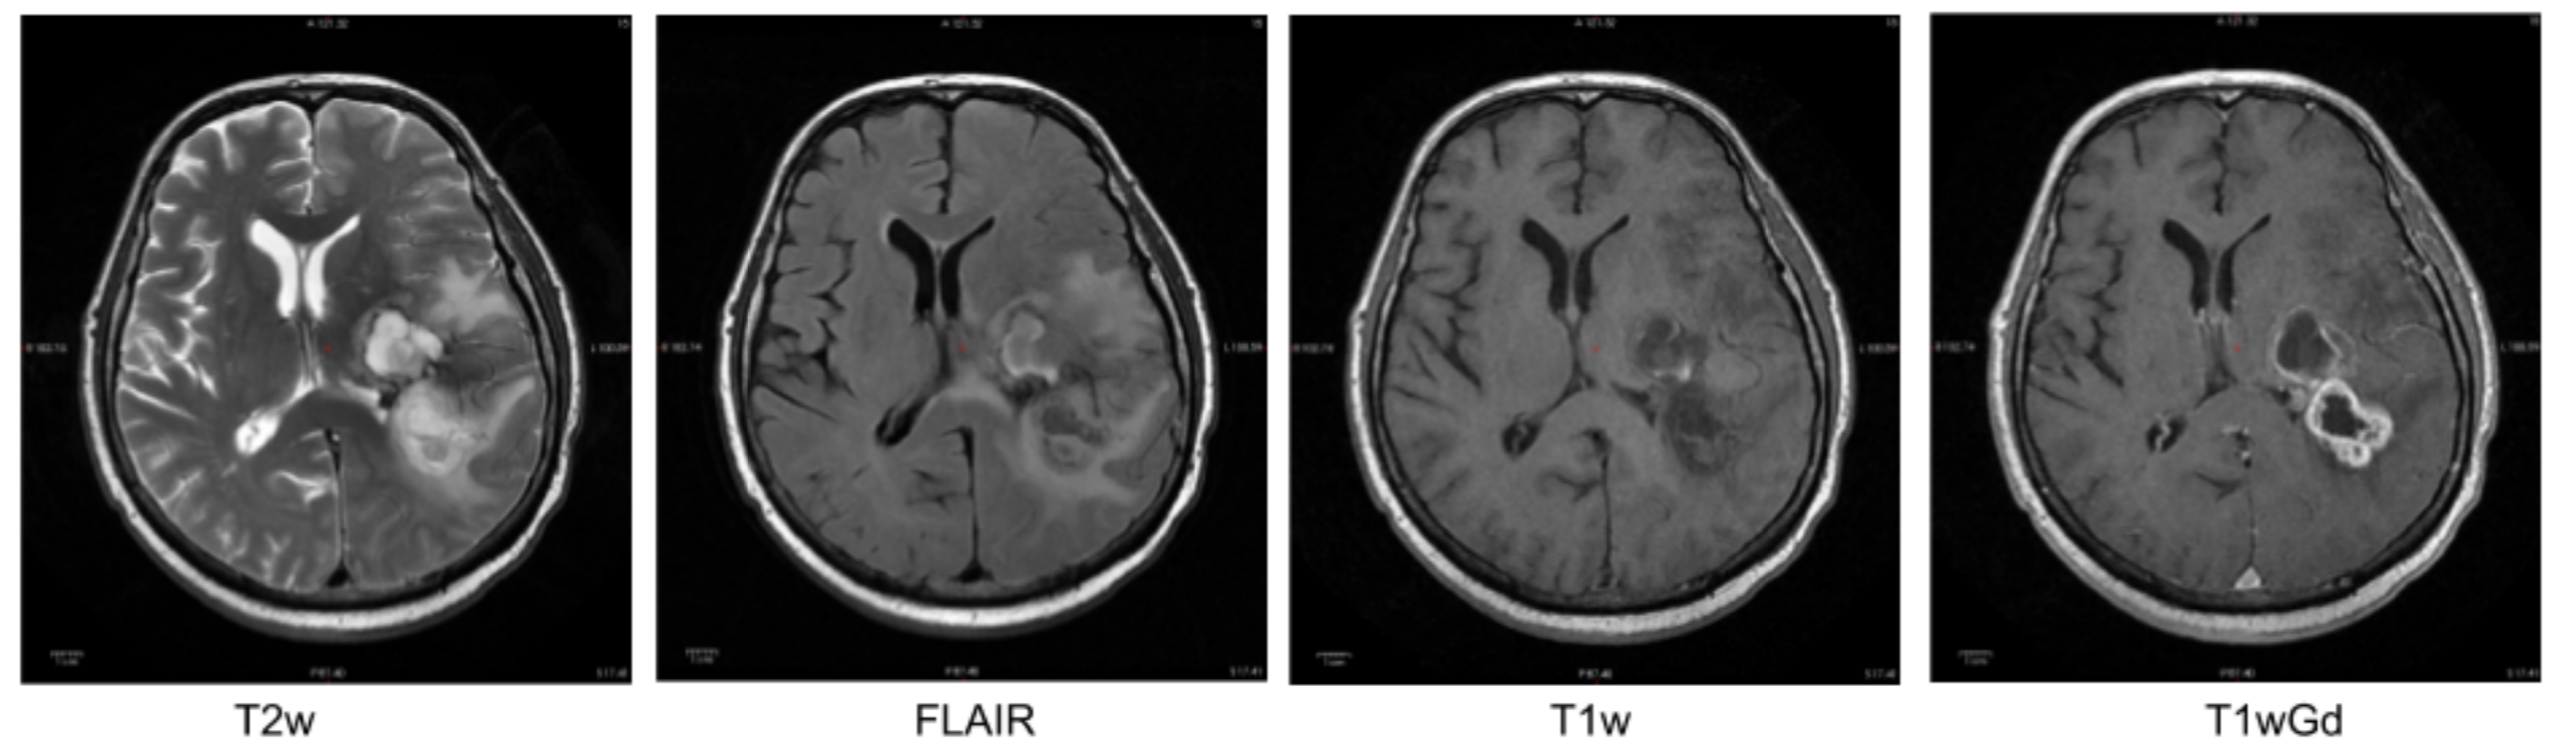
\includegraphics[width=0.9\textwidth]{elmed219_dummy_fig.png}
\caption{This is an ELMED219 dummy figure. (a) T2w, (b) FLAIR, (c) T1w, (d) T1wGd. (Image taken from study TCGA-06-1802 in the TCGA-GBM data collection [ref \cite{TCGA-GBM} in Section 2])}
\label{fig:elmed219-dummy}
\end{figure}



\subsection{Evaluation}

DUMMY TEXT:
%\lipsum
\lipsum[7]


\begin{footnotesize}
\begin{thebibliography}{14} 

\bibitem{Louis2019} Louis DN, Perry A, Reifenberger G  et al. The 2016 World Health Organization Classification of Tumors of the Central Nervous System: a summary. Acta Neuropathol 2016;131:803–820.\\ \scriptsize{\url{https://doi.org/10.1007/s00401-016-1545-1}}

\bibitem{Aldape2019} Aldape K, Brindle KM, Chesler L et al. Challenges to curing primary brain tumours. Nat Rev Clin Oncol 2019;16:509–520.\\ \scriptsize{\url{https://doi.org/10.1038/s41571-019-0177-5}}

% Add references being used

\end{thebibliography}
\end{footnotesize}

\newpage

\section{Data management plan and ethical considerations}
% 1 1/2-2 1/2 pages incl. graphics / links

\subsection{Description of generated data and code}

We will be using data from the TCGA-GBM data collection \cite{TCGA-GBM} ...
DUMMY TEXT:
%\lipsum
\lipsum[8]

\subsection{Sharing of data and code}

DUMMY TEXT:
%\lipsum
\lipsum[9]

\subsection{Ethical considerations}

According to Vollmer et al. \cite{Vollmer2020} ...
DUMMY TEXT:
%\lipsum
\lipsum[10]


\begin{footnotesize}
\begin{thebibliography}{2}

\bibitem{TCGA-GBM} The TCGA-GBM data collection. Accessed on 02/01/2022.\\ \scriptsize{\url{https://wiki.cancerimagingarchive.net/display/Public/TCGA-GBM}}

\bibitem{Vollmer2020} Vollmer S, Mateen BA, Bohner G et al. Machine learning and artificial intelligence research for patient benefit: 20 critical questions on transparency, replicability, ethics, and effectiveness. BMJ 2020;368:l6927. \\
\scriptsize{\url{https://www.bmj.com/content/368/bmj.l6927}}

% Add references being used

\end{thebibliography}
\end{footnotesize}

\end{document}
